\subsection{Distribution Transforming Encoder}

\begin{frame}[t]
	\frametitle{DTE}

	\begin{figure}
	\center
	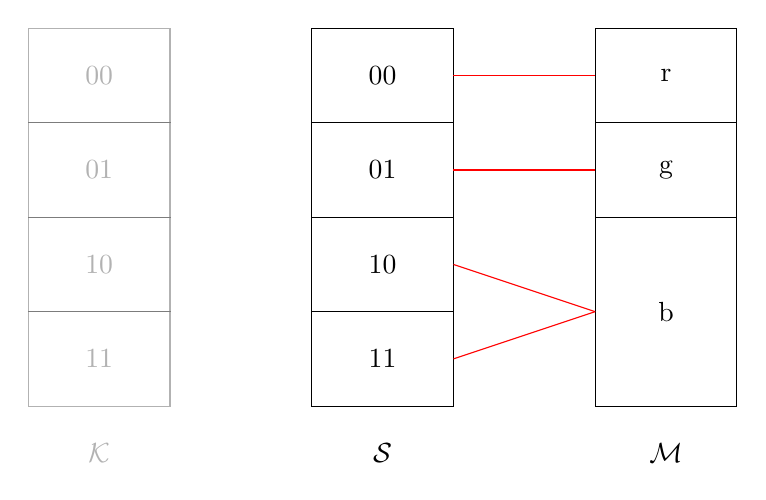
\begin{tikzpicture}[scale=0.6]
		% Linker Kasten
		\begin{scope}[opacity = 0.3]
			\draw (1, 8) rectangle ++ (3, 2) node [midway] {$00$};
			\draw (1, 6) rectangle ++ (3, 2) node [midway] {$01$};
			\draw (1, 4) rectangle ++ (3, 2) node [midway] {$10$};
			\draw (1, 2) rectangle ++ (3, 2) node [midway] {$11$};
			\node at (2.5, 1) {$\mathcal{K}$};
		\end{scope}
		% Mittlerer Kasten
		\begin{scope}
			\draw (7, 8) rectangle ++ (3, 2) node [midway] {$00$};
			\draw (7, 6) rectangle ++ (3, 2) node [midway] {$01$};
			\draw (7, 4) rectangle ++ (3, 2) node [midway] {$10$};
			\draw (7, 2) rectangle ++ (3, 2) node [midway] {$11$};
			\node at (8.5, 1) {$\mathcal{S}$};
		\end{scope}
		% Rechter Kasten
		\begin{scope}
			\draw (13, 8) rectangle ++ (3, 2) node [midway] {r};
			\draw (13, 6) rectangle ++ (3, 2) node [midway] {g};
			\draw (13, 2) rectangle ++ (3, 4) node [midway] {b};
			\node at (14.5, 1) {$\mathcal{M}$};
		\end{scope}
		% Linien
		\draw [color = red] (10, 9) --++ (3, 0);
		\draw [color = red] (10, 7) --++ (3, 0);
		\draw [color = red] (10, 5) --++ (3, -1);
		\draw [color = red] (10, 3) --++ (3, 1);
	\end{tikzpicture}
	\end{figure}

\end{frame}

\begin{frame}[t]
	\frametitle{DTE}

	$$DTE = (encode, decode)$$
	
	\begin{itemize}
		\item $encode$ meist randomisiert
		\item $decode$ deterministisch
	\end{itemize}
	
	\begin{figure}
	\center
	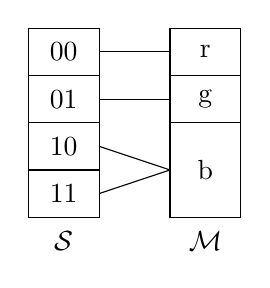
\begin{tikzpicture}[scale=0.3]
		% Mittlerer Kasten
		\begin{scope}
			\draw (7, 8) rectangle ++ (3, 2) node [midway] {$00$};
			\draw (7, 6) rectangle ++ (3, 2) node [midway] {$01$};
			\draw (7, 4) rectangle ++ (3, 2) node [midway] {$10$};
			\draw (7, 2) rectangle ++ (3, 2) node [midway] {$11$};
			\node at (8.5, 1) {$\mathcal{S}$};
		\end{scope}
		% Rechter Kasten
		\begin{scope}
			\draw (13, 8) rectangle ++ (3, 2) node [midway] {r};
			\draw (13, 6) rectangle ++ (3, 2) node [midway] {g};
			\draw (13, 2) rectangle ++ (3, 4) node [midway] {b};
			\node at (14.5, 1) {$\mathcal{M}$};
		\end{scope}
		% Linien
		\draw (10, 9) --++ (3, 0);
		\draw (10, 7) --++ (3, 0);
		\draw (10, 5) --++ (3, -1);
		\draw (10, 3) --++ (3, 1);
	\end{tikzpicture}
	\end{figure}	
	
\end{frame}

\begin{frame}
	\frametitle{DTE}
	Mögliche DTE-Formen:
	
	\begin{itemize}
		\item Tabelle/Datenstruktur zum Nachschauen
	\end{itemize}
	
	\center
	\begin{tabular}{|c|c|}
		\hline
		\textbf{Seed} & \textbf{Nachricht} \\
		\hline
		00 & rot\\
		\hline
		01 & grün\\
		\hline
		10, 11 & blau\\
		\hline
	\end{tabular}
	
	\begin{itemize}
		\item Funktion zur Berechnung
	\end{itemize}
		
			
\end{frame}

\begin{frame}[t]
	\frametitle{DTE}

	Bekannt sein muss:
	\begin{itemize}
		\item Menge/Struktur der Nachrichten
		\begin{itemize}
			\item endlich speicherbar/berechenbar
			\item unendlich berechenbar
		\end{itemize}
		\item Verteilung der Nachrichten
		\begin{itemize}
			\item Nachricht wahrscheinlicher $\Rightarrow$ mehr Seeds
		\end{itemize}
	\end{itemize}

	\begin{figure}
	\center
	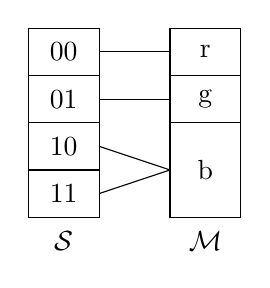
\begin{tikzpicture}[scale=0.3]
		% Mittlerer Kasten
		\begin{scope}
			\draw (7, 8) rectangle ++ (3, 2) node [midway] {$00$};
			\draw (7, 6) rectangle ++ (3, 2) node [midway] {$01$};
			\draw (7, 4) rectangle ++ (3, 2) node [midway] {$10$};
			\draw (7, 2) rectangle ++ (3, 2) node [midway] {$11$};
			\node at (8.5, 1) {$\mathcal{S}$};
		\end{scope}
		% Rechter Kasten
		\begin{scope}
			\draw (13, 8) rectangle ++ (3, 2) node [midway] {r};
			\draw (13, 6) rectangle ++ (3, 2) node [midway] {g};
			\draw (13, 2) rectangle ++ (3, 4) node [midway] {b};
			\node at (14.5, 1) {$\mathcal{M}$};
		\end{scope}
		% Linien
		\draw (10, 9) --++ (3, 0);
		\draw (10, 7) --++ (3, 0);
		\draw (10, 5) --++ (3, -1);
		\draw (10, 3) --++ (3, 1);
	\end{tikzpicture}
	\end{figure}	
	
\end{frame}